\documentclass[a4paper, 12pt]{article}
\usepackage{geometry}
\geometry{margin=1.5cm}

\usepackage[utf8]{inputenc}
\usepackage[russian]{babel}

\usepackage{amsmath, amsfonts, amssymb, amsthm, mathtools}
\usepackage{float}
\usepackage{graphicx}
\usepackage{wrapfig}
\usepackage{subcaption}
\usepackage{pdfpages}

\usepackage{fancyhdr}
\pagestyle{empty}

\usepackage{listings}
\lstnewenvironment{code}{\lstset{
		backgroundcolor=\color{blue!20},
		breaklines=true
}}{}


%\usepackage{fancyvrb,newverbs,xcolor}
%\colorlet{cverbbg}{blue!20}
%\newenvironment{lcverbatim}
%{\SaveVerbatim{cverb}}
%{\endSaveVerbatim
%	\flushleft\fboxrule=0pt\fboxsep=.5em
%	\colorbox{cverbbg}{%
%		\makebox[\dimexpr\linewidth-2\fboxsep][l]{\BUseVerbatim{cverb}}%
%	}
%	\endflushleft
%}

\usepackage{tikz}

\usepackage[pdftex,
					  pdfauthor={Yaroslav Pozdnyak \& Azamat Gimaev},
					  pdftitle={Design},
					  colorlinks=true,
					  linkcolor=blue,
					  filecolor=magenta,      
					  urlcolor=red]{hyperref}


\usepackage{manual}
\usepackage{design}

\def \gitref {https://github.com/gimaevazamat/Design}


\usetikzlibrary{shadings}
\pgfdeclareverticalshading{mygradient}{2cm}{color(0cm)=(blue!50!cyan); color(1.5cm)=(white); color(2.5cm)=(white)}

\begin{document}
%	\begin{tikzpicture}[>=latex']
%		\draw[] (0,0) rectangle (4,4);
%%		\fill[ground] (0,2) arc (23.6:-23.6:5) -- ++ (0.1,0) arc (-23.6:23.6:5);
%	\end{tikzpicture}
	
\begin{huge}
	\begin{center}
		\textbf{Физический рисунок}\\
		\small \textit{by Yaroslav Pozdnyak} \& \textit{Azamat Gimaev} \\
		\large v1.1. Актуальная версия \href{\gitref}{здесь}
	\end{center}
\end{huge}

\section{Общие положения}

\subsection{Начало работы}
Для начала надо \href{\gitref}{отсюда} скачать \verb|design.sty| в директорию вашего документа для использование наших предопределенных команд и стилей

Рисунки выполняются в окружении \verb|tikzpicture|, которое можно встраивать внутрь \verb|figure|:
\begin{code}
	% in preamble: 
	\usepackage{design}
	
	% in document:
	\begin{figure}[H]
		\centering	
		\begin{tikzpicture}
			\draw (0,0) -- (2,0);
		\end{tikzpicture}
	\end{figure}
\end{code}
Этот кусок кода рисует отрезок соединяющий точки с координатами $(0,0)$ и $(2~\text{сm},0)$. Стандартной единицой длины в tikz являются сантиметры, но можно, например, в качестве координаты точки использовать $(2\text{pt}, 0)$.
	

\subsection{Стрелочки и подписи}
Для стрелочек используются аргумент \verb|[>=latex']|, который можно указывать непосредственно при отрисовке каждого объекта, но проще его вынести в аргумент всего изображения:
\begin{code}
	\begin{tikzpicture}[>=latex']
		\draw[->,>=latex'] (0,0) -- ++(2,0);
		\draw (0,0) -- ++ (2/2,0) node [below] {Правильная стрелочка};
	\end{tikzpicture}
\end{code}
Также здесь продемонстрирован пример подписи объекта с использованием команды \verb|node|. Запись \verb|++(2,0)| означает сдвиг отнсительно предыдущей координаты на $2~\text{см}$ вдоль горизонтальной оси .

\begin{figure}[H]
	\centering
	\begin{tikzpicture}[example]
		\draw[->,>=latex'] (0,0) -- ++(2,0);
		\draw (1,0) node [below] {Правильная стрелочка};
		\draw[->] (6,0) -- ++(2,0);
		\draw (7,0) node [below] {Неправильная стрелочка};
	\end{tikzpicture}
\end{figure}

\subsection{Преобразования координат}
Наболее общие линейное преобразование объекта можно сделать с помощью матрицы преобразования.
\begin{figure}[h]
\begin{minipage}{0.3\linewidth}
	\centering
	\begin{tikzpicture}[example]
		\draw(0,0) rectangle (1,1) node[pos=0.5] {$1$};
		\begin{scope} [cm={1,0,.5,.5,(1.5,0)}]
			\draw(0,0) rectangle (1,1) node[pos=0.5] {$2$};
		\end{scope}
		\begin{scope} [cm={.5,.5,0,1,(3.5,0)}]
			\draw(0,0) rectangle (1,1) node[pos=0.5] {$3$};
		\end{scope}
	\end{tikzpicture}
\end{minipage}
\begin{minipage}{0.7\linewidth}
	\begin{code}
	\draw(0,0) rectangle (1,1) node[pos=0.5] {$1$};
	\begin{scope}[cm={1,0,.5,.5,(1.5,0)}]
		\draw(0,0) rectangle (1,1) node[pos=0.5] {$2$};
	\end{scope}
	\begin{scope}[cm={.5,.5,0,1,(3.5,0)}]
		\draw(0,0) rectangle (1,1) node[pos=0.5] {$3$};
	\end{scope}
	\end{code}
\end{minipage}
\end{figure}

Матрицы преобразований, используемые выше:
\[ M_2 = 
\begin{pmatrix}
	1&0\\0.5&0.5
\end{pmatrix}
\quad
M_3 = 
\begin{pmatrix}
	0.5&0.5\\0&1
\end{pmatrix},\]
а сдвиги $\Delta_2=(2,0)$ и $\Delta_3=(4.5,0)$.

\subsection{Запоминание точки}
При создании рисунков бывает удобно запомнить некоторую точку, которая часто будет использоваться в дальнейшем. Это позволит при необходимости быстро и легко поменять координаты в одном месте кода, а не изменять у каждого элемента по-отдельности, в примере ниже медиана $BM$ отрисуется автоматически при изменении координат \verb|(A), (B), (C)|


\begin{figure}[H]
	\begin{minipage}{0.4\linewidth}
		\centering
		\begin{tikzpicture}[example]
			\coordinate (A) at (1,5);
			\draw (A) node[left] {$A$} -- (1.5,3) coordinate (B) node[below left] {$B$}-- (5, 2) coordinate (C) node[right] {$C$}-- (A);	
			
			\draw[red, ultra thick] (B) -- ($(A)!0.5!(C)$) node[above right, black] {$M$};
		\end{tikzpicture}
	\end{minipage}

		\begin{code}
	\coordinate (A) at (1,5);
	\draw (A) node[left] {$A$} -- (1.5,3) coordinate (B) node[below left] {$B$} 
		-- (5, 2) coordinate (C) node[right] {$C$} -- (A);	
	
	% Медиана BM
	\draw[red, ultra thick] (B) -- ($(A)!0.5!(C)$) node[above right, black] {$M$};
		\end{code}

\end{figure}


\subsection{Повороты координат}
Если значительная часть картинки должна быть сдвинута и повернута, то можно использовать окружение \verb|scope|, и использовать аргумент \verb|[shift={(x,y)},rotate=z]|, где \verb|x,y| -- положение центра координат \verb|scope| на холста, а \verb|z| -- угол в градусах, на который будет повернуты координаты внутри \verb|scope| относительно координат \verb|scope|.

\begin{figure}[h]
\begin{minipage}{0.3\linewidth}
	\centering
	\begin{tikzpicture}[example,>=latex', scale=1.5]
		\draw[fill=black!25] (0,0) -- (2,0) -- (20:1) -- cycle;
		\begin{scope}[rotate=20]
			\draw[fill=black!25] (0,0) -- (1.5,0) -- (20:.75) -- cycle;
			\path (20:.75) coordinate (a);
		\end{scope}
		\begin{scope}[shift={(1,0)},rotate=-20]
			\draw[fill=black!25] (0,0) -- (1.5,0) -- (20:.75) -- cycle;
		\end{scope}
		
		\draw[->](a) --++ (0,1);
	\end{tikzpicture}
\end{minipage}
\begin{minipage}{0.7\linewidth}
	\begin{code}
	\draw[fill=black!25] (0,0) -- (2,0) -- (20:1) -- cycle;
	\begin{scope}[rotate=20]
		\draw[fill=black!25] (0,0) -- (1.5,0) -- (20:.75) -- cycle;
		\path (20:.75) coordinate (a);
	\end{scope}
	\begin{scope}[shift={(1,0)},rotate=-20]
		\draw[fill=black!25] (0,0) -- (1.5,0) -- (20:.75) -- cycle;
	\end{scope}
		
	\draw[->](a) --++ (0,1);
	\end{code}
\end{minipage}
\end{figure}

В виде \verb|(20:1)| задается точка, удаленная на расстояние $1~\text{cm}$ от начала отсчета, такая, что ее радиус-вектор составляет угол $20^\circ$ с направлением оси $x$ по часовой стрелке. Также корректно использовать \verb| ++(20:1)| -- сдвиг от текущего положения на $1~\text{cm}$ в направлении составлющем $20^\circ$ с осью $x$.


\subsection{Общий принцип}
Рекомендуется использовать такой принцип работы с жирными линями: какие-то виртуально существующие линии рисовать толщиной \verb|ultrathin|, а физически существующие объекта линиями стандартной толщины либо \verb|thick|. Исключением являются оси систем координат и векторы --- они рисуются линиями стандартной толщины.

\section{Механика}

\subsection{Подвижные тела}
\begin{figure}[H]
	\begin{minipage}{0.4\linewidth}
	\centering
	\begin{tikzpicture}[example]
		\draw (0,0) rectangle (2,1);
		\draw[fill=black!25] (3,0) rectangle (5,1);
	\end{tikzpicture}
\end{minipage}
\begin{minipage}{0.6\linewidth}
	\begin{code}
	\draw (0,0) rectangle (2,1);
	\draw[fill=black!25] (3,0) rectangle (5,1);
	\end{code}
\end{minipage}
\end{figure}



\subsection{Недвижимость}
\begin{figure}[H]
	\begin{minipage}{0.4\linewidth}
		\centering	
		\begin{tikzpicture}[example, >=latex']
			\draw[thick] (0,0) -- (4,0);
			\draw[ground] (0,0) rectangle (4,0.1);
			
			\draw[ultra thin] (0, 0.1) --++ (-0.6,0);
			\draw[ultra thin] (0, 0) --++ (-0.6,0);
			
			\draw[<-,ultra thin] (-0.5, 0.1) --++ (0,0.2);
			\draw[<-,ultra thin] (-0.5, 0) --++ (0,-0.2);
			
			\draw(-0.6,0.1/2) node [left] {$0.1~\text{cm}$};
			
		\end{tikzpicture}
\end{minipage}
\begin{minipage}{0.6\linewidth}
	\begin{code}
	\draw[thick] (0,0) -- (4,0);
	\draw[ground] (0,0) rectangle (4,0.1);
	\end{code}
\end{minipage}
\end{figure}
\begin{figure}[H]
	\begin{minipage}{0.4\linewidth}
	\centering	
	\begin{tikzpicture}[example,>=latex']
		\draw[thick] (0,0) rectangle (4,1);
		\draw[ground] (0,0) rectangle (4,1);
	\end{tikzpicture}
\end{minipage}
\begin{minipage}{0.6\linewidth}
\begin{code}
	\draw[thick] (0,0) rectangle (4,1);
	\draw[ground] (0,0) rectangle (4,1);
\end{code}
\end{minipage}
\end{figure}

\begin{figure}[H]
	\begin{minipage}{0.05\linewidth}
		\centering	
		\begin{tikzpicture}[example,>=latex']
			\begin{scope}[shift={(6,3.23)}]
				\draw(0,0) -- (0.1, 0.173) -- (-0.1, 0.173) -- cycle;
				\draw[thick] (-0.15, 0.173) --++ (0.3, 0);
				\draw[pattern={Lines[angle=45,distance=0.05cm]},fill,draw=none] (-0.15, 0.173) rectangle ++(0.3, 0.1);
			\end{scope}
		\end{tikzpicture}
	\end{minipage}
	\begin{minipage}{0.95\linewidth}
		\begin{code}
	\begin{scope}[shift={(x, y)}] %(x, y) – координаты нижней вершины треугольника
		\draw(0,0) -- (0.1, 0.173) -- (-0.1, 0.173) -- cycle;
		\draw[thick] (-0.15, 0.173) --++ (0.3, 0);
		\draw[pattern={Lines[angle=45,distance=0.05cm]},fill,draw=none] (-0.15, 0.173) rectangle ++(0.3, 0.1);
	\end{scope}
		\end{code}
	\end{minipage}
\end{figure}
\subsection{Подвижное тело на недвижимости}
Чтобы подчеркнуть подвижность тела, можно добавить расстоние $0.025~\text{cm}$, чтобы оно <<парило>> над поверхностью:

\begin{figure}[H]
	\centering	
	\begin{tikzpicture}[example, >=latex']
		\draw[thick] (-1,0) -- (1,0);
		\fill[ground] (-1,-0.1) rectangle (1,0);
		
		\draw(-0.5,0.025) rectangle ++(1,1);
	\end{tikzpicture}
\end{figure}

\subsection{Пружины}
\begin{figure}[H]
	\begin{minipage}{0.5\linewidth}
	\centering	
	\begin{tikzpicture}[example, >=latex']
		\draw[decorate,decoration=
		{snake,pre length=0.5cm,post length=0.5cm,segment length=0.25cm,amplitude=0.25cm}]
		(0,0) -- (4,0);
		
		\draw[ultra thin] (0,0.25) -- ++ (0,.6);
		\draw[ultra thin] (0.5,0.25) -- ++ (0,.6);
		\draw[ultra thin, <->] (0,0.25+0.5) -- (0.5/2,0.25+0.5) node [above] {pre length} -- (0.5,0.25+0.5);
		
		\draw[ultra thin] (3.5,0.25) -- ++ (0,.6);
		\draw[ultra thin] (4,0.25) -- ++ (0,.6);
		\draw[ultra thin, <->] (3.5,0.25+0.5) -- (3.5+0.5/2,0.25+0.5) node [above] {post length} -- (3.5+0.5,0.25+0.5);
		
		\draw[ultra thin] (2-0.05,-0.25) -- ++ (0,-.6);
		\draw[ultra thin] (2-0.05+0.25,-0.25) -- ++ (0,-.6);
		\draw[ultra thin,<-] (2-0.05,-0.25) ++ (0,-.5) -- ++ (-0.2,0);
		\draw[ultra thin,<-] (2-0.05+0.25,-0.25) ++ (0,-.5) -- ++ (0.2,0);
		\draw (2-0.05+0.25/2,-0.25) ++ (0,-.6) node [below] {segment length};
		
		\draw[ultra thin] (0,0.25) -- ++ (-0.6,0);
		\draw[ultra thin] (0,0) -- ++ (-0.6,0);
		\draw[ultra thin,<-] (0,0.25) ++ (-0.5,0) -- ++ (0,0.2);
		\draw[ultra thin,<-] (0,0) ++ (-0.5,0) -- ++ (0,-0.2);
		\draw(0,0.25/2) ++ (-0.6,0) node [left] {amplitude};
		
		
	\end{tikzpicture}
\end{minipage}
\begin{minipage}{0.5\linewidth}
\begin{code}
	\draw[decorate,decoration={snake,
		pre length=0.5cm, post length=0.5cm,
		segment length=0.5cm,
		amplitude=0.25cm}]
	(0,0) -- (4,0);
\end{code}
\end{minipage}
\end{figure}

\subsection{Жидкости, сосуды и поршни}
\begin{enumerate}
	\item Сосуды рисуются \verb|thick| линиями.
	\item Для отрисовки воды используется аргумент \verb|water|, которые автоматически заливает фигуру голубым полупрозрачным цветом. Также есть предопределенные цвета для других заливок: \verb|gas|, \verb|glass|, \verb|oil|
	\item Поршни выделются серым \verb|black!25| цветом.
	\item Зазор между поршнем и стенками сосуда 0.025 cm
\end{enumerate}

\begin{figure}[H]
	\begin{minipage}{0.2\linewidth}
	\centering	
	\begin{tikzpicture}[example, >=latex']
		\fill[water] (0,-.5) rectangle ++(2,-2.5);
		
		\draw[fill=black!25] (0.025,-0.5) rectangle ++(2-0.05,0.1);
		\draw[thick] (1,-0.4) -- ++(0,1);
		
		\draw[thick] (0,0) --++(0,-3) --++(2,0) --++(0,3);	
	\end{tikzpicture}
\end{minipage}
\begin{minipage}{0.8\linewidth}
\begin{code}
	\fill[water] (0,-.5) rectangle ++(2,-2.5);
	
	\draw[fill=black!25] (0.025,-0.5) rectangle ++(2-0.05,0.1);
	\draw[thick] (1,-0.4) -- ++(0,1);
	
	\draw[thick] (0,0) --++(0,-3) --++(2,0) --++(0,3);	
\end{code}
\end{minipage}
\end{figure}

\subsection{Блоки и нити}

Центр блока обозначается белым кругом радиуса 0.05 cm. Нити рисуются линиями стандартной толщины, для блоков используется \verb|thick|.
\begin{figure}[H]
	\begin{minipage}{0.2\linewidth}
	\centering	
	\begin{tikzpicture}[example, >=latex']
		\draw[thick] (0,0) circle (0.5);
		\draw (0,0) circle (0.05);
		\draw (0,0.05) -- (0,2);
		
		\path[rotate=30] (0.5,0) coordinate (a);
		\draw[shift=(a),rotate=30] (0,0) -- (0,-1); 
		
		\draw (-0.5,0) -- ++(0,-1);
	\end{tikzpicture}
\end{minipage}
\begin{minipage}{0.8\linewidth}
\begin{code}
	\draw[thick] (0,0) circle (0.5);
	\draw (0,0) circle (0.05);
	
	\draw (0,0.05) -- (0,2); %нить, на которой подвешен блок
	
	\path[rotate=30] (0.5,0) coordinate (a);
	\draw[shift=(a),rotate=30] (0,0) -- (0,-1);  %правая нить
	
	\draw (-0.5,0) -- ++(0,-1); %левая нить
\end{code}
\end{minipage}
\end{figure}

\subsection{Гирька}
Если в Вашем рисунке присутствует гирька, то Вы можете воспользоваться этим паттерном:

\begin{figure}[H]
	\begin{minipage}{0.07\linewidth}
		\centering	
		\begin{tikzpicture}[example, >=latex']
			\draw[fill=black!25](-.2,0) -- (-.2,.3) .. controls (0,.4) and (-.1,.4) .. (-.1,.5) arc (180:0:.1) .. controls (.1,.4) and (0,.4) .. (.2,.3) -- (.2,0) -- cycle;
		\end{tikzpicture}
	\end{minipage}
	\begin{minipage}{0.93\linewidth}
\begin{code}
	\draw[fill=black!25](-.2,0) -- (-.2,.3) .. controls (0,.4) and (-.1,.4).. (-.1,.5) arc (180:0:.1) .. controls (.1,.4) and (0,.4) .. (.2,.3) -- (.2,0) -- cycle;
\end{code}
	\end{minipage}
\end{figure}

\subsection{Гайка}
Если в Вашем рисунке присутствует гайка, то Вы можете воспользоваться этим паттерном. \verb|(x, y)| -- координата середины гайки.

\begin{figure}[H]
	\begin{minipage}{0.07\linewidth}
		\centering	
		\begin{tikzpicture}[example, >=latex']
			\begin{scope}[shift={(0,0)}, scale=0.4]
				\draw[fill=black!25](-0.5, -0.866) -- (0.5, -0.866) -- (1, 0) -- (0.5, 0.866) -- (-0.5, 0.866) -- (-1, 0) -- cycle;
				\draw[fill=yellow!20] (0, 0) circle(0.45);
			\end{scope}
		\end{tikzpicture}
	\end{minipage}
	\begin{minipage}{0.93\linewidth}
		\begin{code}
	\begin{scope}[shift={(x, y)}, scale=0.4]
		\draw[fill=black!25](-0.5, -0.866) -- (0.5, -0.866) -- (1, 0) -- (0.5, 0.866) -- (-0.5, 0.866) -- (-1, 0) -- cycle;
		\draw[fill=white] (0, 0) circle(0.45);
	\end{scope}
		\end{code}
	\end{minipage}
\end{figure}



\section{Выносные размеры}
\subsection{Линейные размеры}
В стандартных случаях, как например подпись длины прямоугольника, можно использовать команды \verb|\dist| и \verb|\sdist|:
\begin{figure}[H]
\begin{minipage}{0.4\linewidth}
		\centering	
	\begin{tikzpicture}[example, >=latex']
		\draw (0,0) rectangle (4,0.5);
		
		\dist{(0, 0.5)}{(4, 0.5)}{90}{above}{4 cm}
		\sdist{(0,0)}{(0,0.5)}{180}{left}{0.5 cm}
	\end{tikzpicture}
\end{minipage}
\begin{minipage}{0.6\linewidth}
\begin{code}
	\dist{(0, 0.5)}{(4, 0.5)}{90}{above}{4 cm}
	
	\sdist{(0,0)}{(0,0.5)}{180}{left}{0.5 cm}
\end{code}
\end{minipage}
\end{figure}

\begin{figure}[H]
\begin{minipage}{0.4\linewidth}
	\centering	
	\begin{tikzpicture}[example, >=latex']
		\draw (0,0) rectangle (4,0.5);
		
		\dist[1][0.7]{(0, 0.5)}{(4, 0.5)}{90}{above}{4 cm}
		\sdist[1.5][0.3]{(0,0)}{(0,0.5)}{180}{left}{0.5 cm}
	\end{tikzpicture}
\end{minipage}
\begin{minipage}{0.6\linewidth}
	\begin{code}
	\dist[1][0.7]{(0,0.5)}{(4,0.5)}{90}{above}{4cm}

	\sdist[1.5][0.3]{(0,0)}{(0,0.5)}{180}{left}{0.5 cm}
	\end{code}
\end{minipage}
\end{figure}

Команды \verb|\dist| и \verb|\sdist| имеют 5 обязательных (указываются в фигурных скобках \verb|{}|) и 2 опциональных аргумента (указываются в квадратных скобках \verb|[]| \textbf{перед обязательными}). 
\begin{itemize}
	\item Первый опциональный аргумент -- это длина выносной линии в сантиметрах\\(\verb|default = 0.6 cm|)
	\item Второй -- расстояние от стрелок до точек, куда подносится выносной размер\\(\verb|default = 0.5 cm|)
	\item Первые два обязательных аргумента -- это точки, к которым мы хотим поднести наш выносной размер(указываются обе координаты в круглых скобках \verb|(x, y)|)
	\item Третий обязательный аргумент -- это угол в градусах, на который повернуты габартиные линии
	\item Четвертый обязательный аргумент -- это расположение подписи, относительно центра линии, соединяющей стрелочки (\verb|above, below, right, left|)
	\item Пятый обязательный аргумент -- это текст подписи
\end{itemize}

\subsection{Угловые размеры}
Для указания угловых размеров обычно удобно использовать следующие параметры: радуиус дуги $0.75~\text{cm}$, расстояние до подписи $1.0~\text{cm}$.

\begin{figure}[H]
\begin{minipage}{0.2\linewidth}
	\centering	
\begin{tikzpicture}[example, >=latex']
	\draw (0,0) -- (2,0);
	\draw[rotate=30] (0,0) -- (2,0);
	\draw[rotate=80] (0,0) -- (2,0);	
	
	\draw(0.75,0) arc (0:30:0.75);
	\path[rotate=30/2] (1,0) node {$\alpha$};
	
	\draw[rotate=30,double=yellow!20](0.75,0) arc (0:50:0.75);
	\path[rotate=30+50/2] (1,0) node {$\beta$};
\end{tikzpicture}
\end{minipage}
\begin{minipage}{0.8\linewidth}
	\begin{code}
	\draw (0,0) -- (2,0);
	\draw[rotate=30] (0,0) -- (2,0);
	\draw[rotate=80] (0,0) -- (2,0);	
	
	%дуга 0-30
	\draw(0.75,0) arc (0:30:0.75);
	\path[rotate=30/2] (1,0) node {$\alpha$};
	
	%двойная дуга 30-80
	\draw[rotate=30,double=yellow!20](0.75,0) arc (0:50:0.75);
	\path[rotate=30+50/2] (1,0) node {$\beta$};
	\end{code}
\end{minipage}
\end{figure}



\section{Оптика}
\subsection{Источники света}
Команда \verb|\lightsource| рисует источник света и в качестве аргумента принимает его координаты. Подписи к источникам света удаляются на 0.2 cm.

\begin{figure}[H]
	\begin{minipage}{0.1\linewidth}
	\centering	
	\begin{tikzpicture}[example, >=latex']
		\lightsource{(0,0)};
		\draw (0,0) node [above=0.2cm] {$S$};
	\end{tikzpicture}
\end{minipage}
\begin{minipage}{0.9\linewidth}
\begin{code}
	\lightsource{(0,0)};
	\draw (0,0) node [above=0.2cm] {$S$};
\end{code}
\end{minipage}
\end{figure}


\subsection{Стеклянные объекты}
Аналогично с водой, аргумент \verb|glass| приводит к автоматической полупрозрачной заливки объекта.
\begin{figure}[H]
\noindent\begin{minipage}{0.2\linewidth}
	\centering	
	\begin{tikzpicture}[>=latex']
		\draw[glass] (0,0) rectangle (3,1.5);
	\end{tikzpicture}
\end{minipage}
\begin{minipage}{0.8\linewidth}
\begin{code}
	\draw[glass] (0,0) rectangle (3,1.5);
\end{code}
\end{minipage}
\end{figure}

\subsection{Зеркала и экраны}
Отрисовка экранов и зеркал похожа на отрисовку недвижимости, только надо использовать аргумент \verb|[screen]|. Линия экрана рисуется толщиной \verb|thick|
\begin{figure}[H]
\begin{minipage}{0.15\linewidth}
	\centering	
	\begin{tikzpicture}[example, >=latex']
		\draw[thick] (0,0) -- (0, -5);
		\fill[screen] (0,0) rectangle (0.1, -5);
		
		\draw[thick] (0.7,-0.1) arc (23.6:-23.6:6);
		\fill[screen] (0.7,-0.1) ++(23.6:0.1) arc(23.6:-23.6:6.1) -- ++(-23.6:-0.1) arc (-23.6:23.6:6);
	\end{tikzpicture}
\end{minipage}
\begin{minipage}{0.85\linewidth}
	\begin{code}
	\draw[thick] (0,0) -- (0, -5);
	\fill[screen] (0,0) rectangle (0.1, -5);
	
	\draw[thick] (0.7,-0.1) arc (23.6:-23.6:6);
	\fill[screen] (0.7,-0.1) ++(23.6:0.1) arc(23.6:-23.6:6.1) -- ++(-23.6:-0.1) arc (-23.6:23.6:6);
	\end{code}
\end{minipage}
\end{figure}

Чтобы на рисунках можно было визуально различать зеркала и экраны рекомендуется использовать для зеркал шаблон, представленный ниже. \textbf{Важно} делать заливку до отрисовки линии, иначе часть толщины линии будет перекрыта
\begin{figure}[H]
	\begin{minipage}{0.15\linewidth}
		\centering	
		\begin{tikzpicture}[example]
			\fill[mirror] (0,0) rectangle (0.1, -5);
			\draw[thick] (0,0) -- (0, -5);
			
			\fill[mirror] (0.7,-0.1) ++(23.6:0.1) arc(23.6:-23.6:6.1) -- ++(-23.6:-0.1) arc (-23.6:23.6:6);
			\draw[thick] (0.7,-0.1) arc (23.6:-23.6:6);
		\end{tikzpicture}
	\end{minipage}
	\begin{minipage}{0.85\linewidth}
	\begin{code}
	\fill[mirror] (0,0) rectangle (0.1, -5);
	\draw[thick] (0,0) -- (0, -5);
	
	\fill[mirror] (0.7,-0.1) ++(23.6:0.1) arc(23.6:-23.6:6.1) -- ++(-23.6:-0.1) arc (-23.6:23.6:6);
	\draw[thick] (0.7,-0.1) arc (23.6:-23.6:6);
	\end{code}
	\end{minipage}
\end{figure}


\subsection{Лучи}
Лучи рисуются линиями стандартной толщины.
\begin{figure}[H]
\begin{minipage}{0.2\linewidth}
	\centering	
	\begin{tikzpicture}[example, >=latex']
		\draw (0,0) -- ++ (2,0);
		\draw[directed] (0,-0.5) -- ++ (2,0);
		\draw[reverse directed] (0,-1) -- ++ (2,0);
	\end{tikzpicture}
\end{minipage}
\begin{minipage}{0.8\linewidth}
	\begin{code}
	\draw (0,0) -- ++ (2,0)
	\draw[directed] (0,-0.5) -- ++ (2,0)
	\draw[reverse directed] (0,-1) -- ++ (2,0)
	\end{code}
\end{minipage}

\end{figure}




\section{Электрические схемы}
Для отрисовки электрических схем используется пакет \verb|circuittikz|, у которого есть понятная \href{https://tug.org/docs/latex/circuitikz/circuitikzmanual.pdf}{документация}

Рекомендуется использовать аргументы \verb|european resistors| и \verb|american inductors| у всего рисунка
\begin{code}
%	in preamble:
	\usepackage{circuitikz}
%	in document:
	\begin{tikzpicture}[european resistors, american inductors]
	\end{tikzpicture}
\end{code}

Или можно задать это для всего документа в преамбуле:\\
\begin{code}
%	in preamble:
	\usepackage{circuitikz}
	\ctikzset{resistor = european, inductor = american}
\end{code}

\subsection{Общая логика, провода}
Общая логика пакета \verb|circuittikz| строится вокруг декорирования пути между двумя точками. Для этого используются дополнительные аргументы у команды \verb|to[]|. Для работы с проводами используется аргумент \verb|short|.
\begin{figure}[H]

\begin{minipage}{0.2\linewidth}
	\centering	
	\begin{tikzpicture}[example, european resistors, american inductors]
		\draw (0,0) to ++(1,0);
		\draw (0,-0.5) to[short,-o] ++(1,0);
		\draw (0,-1) to[short,*-] ++(1,0);
		\draw (0,-1.5) to[short,-*] ++(1,0);
		\draw (0,-2) to[short,*-o] ++(1,0);
	\end{tikzpicture}
\end{minipage}
\begin{minipage}{0.8\linewidth}
	\begin{code}
	\draw (0,0) to[short,-] ++(1,0);
	\draw (0,-1) to[short,-o] ++(1,0);
	\draw (0,-2) to[short,*-] ++(1,0);
	\draw (0,-3) to[short,-*] ++(1,0);
	\draw (0,-4) to[short,*-o] ++(1,0);
	\end{code}
\end{minipage}

\end{figure}

\subsection{Резисторы}
Резистору соотвествует аргумент \verb|R|. Потенциометру соотвествует аргумент \verb|pR|.
\begin{figure}[H]
\begin{minipage}{0.2\linewidth}
	\centering	
	\begin{tikzpicture}[example]
		\draw (0,0)
		to[R=$R_1$] ++ (1.5,0);
		
		\draw (0,-2)
		to[pR=$R_2$,name=pR] ++ (1.5,0);
		
		\draw(pR.wiper) to[short,-o] ++(1,0);
	\end{tikzpicture}
\end{minipage}
\begin{minipage}{0.8\linewidth}
	\begin{code}
	\draw (0,0)
	to[R=$R_1$] ++ (1.5,0);
	
	\draw (0,-1.56)
	to[pR=$R_2$,name=pR] ++ (1.5,0);
	
	\draw(pR.wiper) to[short,-o] ++(1,0);
	\end{code}
\end{minipage}

\end{figure}

Для работы с третьим выходом потенциометра даем уникальное название name потенциометру, а далее обращаемся к этой координате, как к \verb|name.wiper| (\textit{в примере выше это} \verb|pR.wiper|).

Параметр \verb|/tikz/circuitikz/bipoles/length=| изменит размер элементов с двумя выводами
\begin{figure}[H]
\begin{minipage}{0.2\linewidth}
	\centering	
	\begin{tikzpicture}[example, european resistors, american inductors]
		\draw (0,0) 
		to [R=$R$, /tikz/circuitikz/bipoles/length=2cm] ++(3,0);
		
		\draw (0.5,-1.5) 
		to [R=$r$, /tikz/circuitikz/bipoles/length=0.5cm] ++(2,0);
	\end{tikzpicture}
\end{minipage}
\begin{minipage}{0.8\linewidth}
	\begin{code}
	\draw (0,0) 
	to [R=$R$, /tikz/circuitikz/bipoles/length=2cm] ++(3,0);
	
	\draw (0.5,-1.5) 
	to [R=$r$, /tikz/circuitikz/bipoles/length=0.5cm] ++(2,0);
	\end{code}
\end{minipage}
\end{figure}

\subsection{Источник напряжения и источник тока}
Источнику постоянного напряжения соотвествует аргумент \verb|battery1|. 
\begin{figure}[H]
\begin{minipage}{0.2\linewidth}
	\centering	
	\begin{tikzpicture}[example, european resistors, american inductors]
		\draw (0,0)
		to[battery1,l=$\mathcal{E}_1$] ++ (1.5,0);
		
		\draw (0,-2)
		to[battery1,l=$\mathcal{E}_2$,invert] ++ (1.5,0);
	\end{tikzpicture}
\end{minipage}
\begin{minipage}{0.8\linewidth}
	\begin{code}
	\draw (0,0)
	to[battery1,l=$\mathcal{E}_1$] ++ (1.5,0);
	
	\draw (0,-2)
	to[battery1,l=$\mathcal{E}_2$,invert] ++ (1.5,0);
	\end{code}
\end{minipage}

\end{figure}

Чтобы развернуть батареку используйте аргумент \verb|invert|. Наименования батареек следует добавлять с помощью дополнительного аргумента \verb|l=label|.

\begin{figure}[H]
	\begin{minipage}{0.2\linewidth}
		\centering
		\begin{tikzpicture}[example]
			\draw (0,0) to[american current source, l=$I_0$] (0,1.5);
		\end{tikzpicture}
	\end{minipage}
	\begin{minipage}{0.8\linewidth}
		\begin{code}
	\draw (0,0) to[american current source, l=$I_0$] (0,1.5);
%	or
	\draw (0,0) to[american, isource, l=$I_0$] (0,1.5);
		\end{code}
	\end{minipage}
\end{figure}
\subsection{Ключи}
Обычному ключу соотвествует аргумент nos.

\begin{figure}[H]

\begin{minipage}{0.2\linewidth}
	\centering	
	\begin{tikzpicture}[example, european resistors, american inductors]
		\draw (0,0)
		to[nos=$K$] ++ (1.5,0);
	\end{tikzpicture}
\end{minipage}
\begin{minipage}{0.8\linewidth}
	\begin{code}
	\draw (0,0)
	to[nos=$K$] ++ (1.5,0);
	\end{code}
\end{minipage}

\end{figure}



\subsection{Конденсаторы, катушки}
Конденсатору соотвествует аргумент \verb|C|. Катушке соотвествует аргумент \verb|L|.
\begin{figure}[H]
\begin{minipage}{0.3\linewidth}
	\centering	
	\begin{tikzpicture}[example]
		\draw (-2.25,0)
		to[C] ++ (1.5,0)
		to[C=$C$] ++ (1.5,0)
		to[C=$C$] ++ (1.5,0);
		
		\draw(0,0) ++ (-.4,.4) node {\small $+$};
		\draw(0,0) ++ (.4,.4) node {\small $-$};
		
		\draw(1.5,0) ++ (-.4,.4) node {\small $q$};
		
		\draw (-.75,-2)
		to[L=$L$] ++ (1.5,0);
	\end{tikzpicture}
\end{minipage}
\begin{minipage}{0.7\linewidth}
\begin{code}
	\draw (-2.25,0)
	to[C] ++ (1.5,0)
	to[C=$C$] ++ (1.5,0)
	to[C=$C$] ++ (1.5,0);
	
	\draw(0,0) ++ (-.4,.4) node {\small $+$};
	\draw(0,0) ++ (.4,.4) node {\small $-$};
	
	\draw(1.5,0) ++ (-.4,.4) node {\small $q$};
	
	\draw (-.75,-2)
	to[L=$L$] ++ (1.5,0);
\end{code}
\end{minipage}
\end{figure}
Иногда в задаче нужно указать знаки либо величины зарядов на пластинах конденсатора. В таком случае используются удаленные от центра конденастора на 0.4 cm метки, сделанные шрифтом \verb|small|.

\subsection{Вольтметры, амперметры, омметры}
Измерительные приборы создаются с помощью аргумента rmeter
\begin{figure}[H]
\begin{minipage}{0.3\linewidth}
	\centering	
	\begin{tikzpicture}[example, european resistors, american inductors]
		\draw (0,0)
		to[rmeter,t=A] (1.5,0)
		to[rmeter,t=V] (3,0)
		to[rmeter,t=$\Omega$] (4.5,0);
		
		\draw(3.75,0) ++ (-.4,.4) node {\small $+$};
	\end{tikzpicture}
\end{minipage}
\begin{minipage}{0.7\linewidth}
	\begin{code}
	\draw (0,0)
	to[rmeter,t=A] (1.5,0)
	to[rmeter,t=V] (3,0)
	to[rmeter,t=$\Omega$] (4.5,0);
	
	\draw(3.75,0) ++ (-.4,.4) node {\small $+$};
	\end{code}
\end{minipage}
\end{figure}

\subsection{Другие элеткрические элементы}

\begin{figure}[H]
	\begin{minipage}{0.3\linewidth}
		\centering	
		\begin{tikzpicture}[example, european resistors, american inductors]
			\draw (1.5,0)
			to[lamp] ++(1.5,0);
			
			\draw (0,-1.5)
			to[diode] ++(1.5,0)
			to[photodiode] ++(1.5,0)
			to[led]++(1.5,0);
			
			\draw (0.75, -3)
			to[memristor] ++(3,0);
									
		\end{tikzpicture}
	\end{minipage}
	\begin{minipage}{0.7\linewidth}
		\begin{code}
	\draw (1.5,0)
	to[lamp] ++(1.5,0);
	
	\draw (0,-1.5)
	to[diode] ++(1.5,0)
	to[photodiode] ++(1.5,0)
	to[led]++(1.5,0);
	
	\draw (0.75,-3)
	to[memristor] ++(3,0);
		\end{code}
	\end{minipage}
\end{figure}

\subsection{Заземление}
\begin{figure}[H]
	\begin{minipage}{0.1\linewidth}
		\centering	
		\begin{tikzpicture}[example, european resistors, american inductors]
			\draw (0,0)
			to (0,-1) node[tlground]{};
		\end{tikzpicture}
	\end{minipage}
	\begin{minipage}{0.9\linewidth}
		\begin{code}
	\draw (0,0)
	to (0,-1) node[tlground]{};
		\end{code}
	\end{minipage}
\end{figure}

\subsection{Сила тока в цепях}
По умолачанию сила тока в пакете \verb|circuittikz| обозначаются и выглядят так:
\begin{figure}[H]
	\begin{minipage}{0.2\linewidth}
		\centering	
		\begin{tikzpicture}[example, european resistors, american inductors]
			\draw (0,0) to[R, i^>=$I_1$] (3,0);
		\end{tikzpicture}
	\end{minipage}
	\begin{minipage}{0.8\linewidth}
		\begin{code}
	\draw (0,0) to[R, i^>=$I_1$] (3,0);			
		\end{code}
	\end{minipage}
\end{figure}

Такой вариант не рекомендуется использовать. Для привычного обозначения можно использовать \verb|flow| (потоки) из этого пакета:

\begin{figure}[H]
	\begin{minipage}{0.4\linewidth}
		\centering	
		\begin{tikzpicture}[example, european resistors, american inductors]
			\draw (0,0) 
			to[R, f^>=$I_2$] ++(3,0)
			to[R, f_>=$I_3$, flow/distance=1] ++(3,0);
		\end{tikzpicture}
	\end{minipage}
	\begin{minipage}{0.6\linewidth}
		\begin{code}
	\draw (0,0) 
	to[R, f^>=$I_2$] ++(3,0)
	to[R, f_>=$I_3$, flow/distance=1] ++(3,0);
		\end{code}
	\end{minipage}
\end{figure}
Аргумент \verb|flow/distance=| меняет расположение стрелочки вдоль провода. Настроить расположение стрелки относительно провода(сверху/снизу) и направление можно используя разные символы после \verb|f|: \verb|f=,  f<=,  f_=, f_>=, f<^=, f<_=, f>_=|

 
\section{Лайфхаки}
\subsection{Вертикальные подписи для электрических схем}
\begin{enumerate}
	\item Чтобы подписи для повернутых элементов были тоже вертикальными пользуйтесь командой
\begin{code}
	\ctikzset{label/align = straight}
\end{code}
	в самом начале кода рисунка.
\end{enumerate}
\subsection{Вставка растрового риснука внутрь tikz}
Если вам, например, понадобилось нарисовать обозначения поверх фотографии, то вы можете вставить избражение внутрь \verb|tikzpicture| с помощью команды \verb|\includegraphics|, как текст \verb|node| выбранная точка будет центром вставленного изображения.

\begin{figure}[H]
\begin{minipage}{0.3\linewidth}
	\centering	
	\begin{tikzpicture}[example,>=latex',scale=4.0/6.0]
	\path (0,0) node {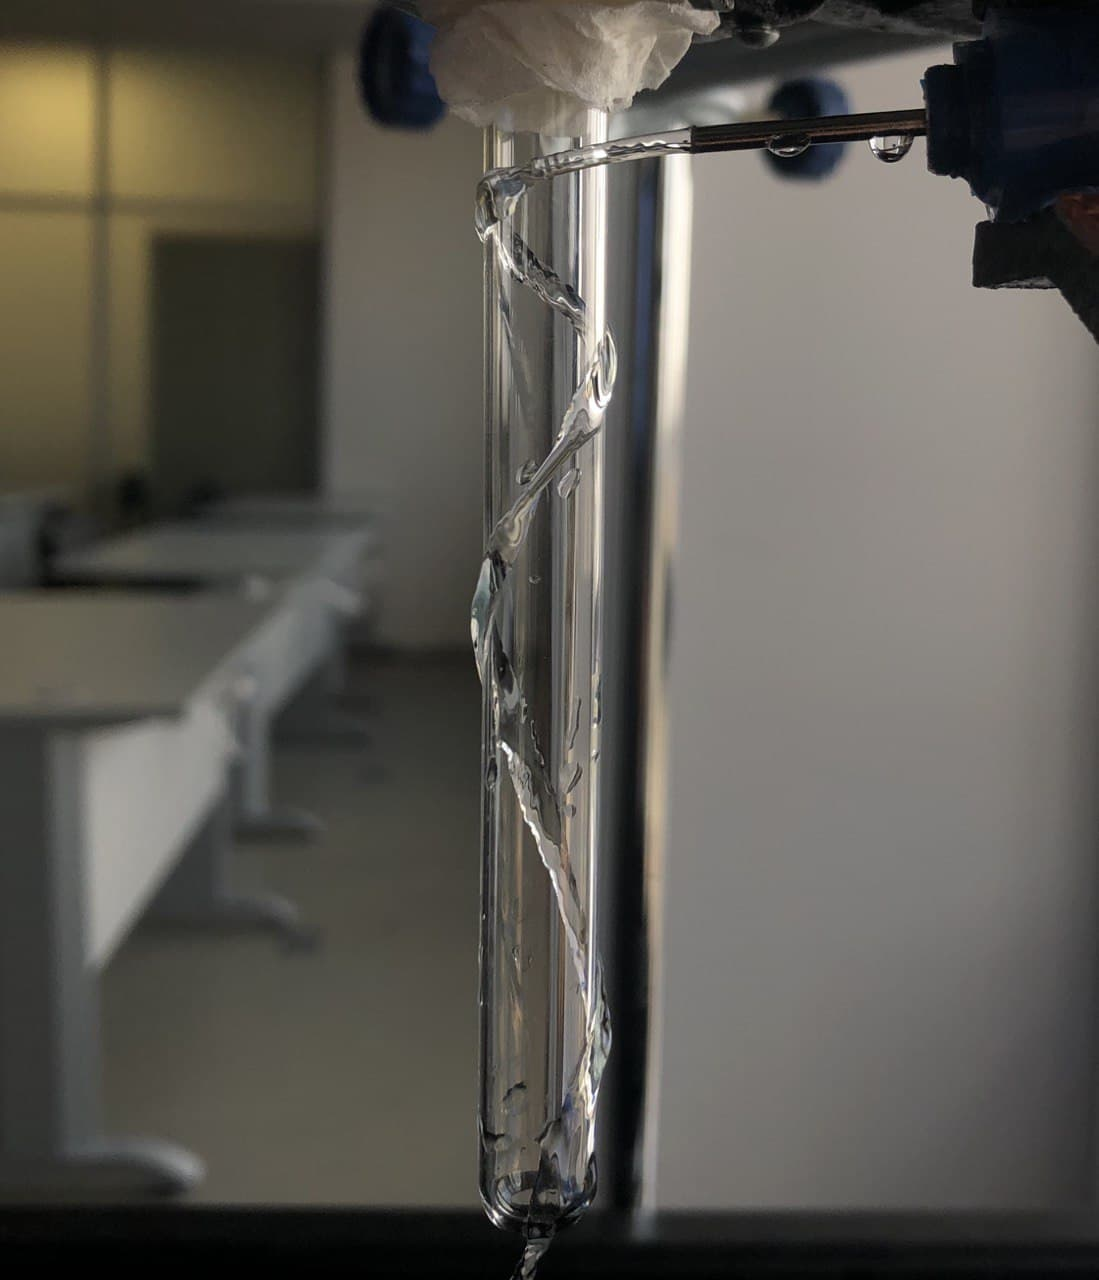
\includegraphics[width=4cm]{pic.jpg}};
    
    \begin{scope}[draw=white]
    		\dist{(0,2.57)}{(0,1.0)}{180}{left}{}
    		\path(0,{(2.57+1.0)/2}) ++ (180:.5) node [left,white] {$\lambda$};
    \end{scope}

	\end{tikzpicture}
\end{minipage}
\begin{minipage}{0.7\linewidth}
	\begin{code}
	\begin{tikzpicture}[example,>=latex',scale=4.0/6.0]
	\path (0,0) node {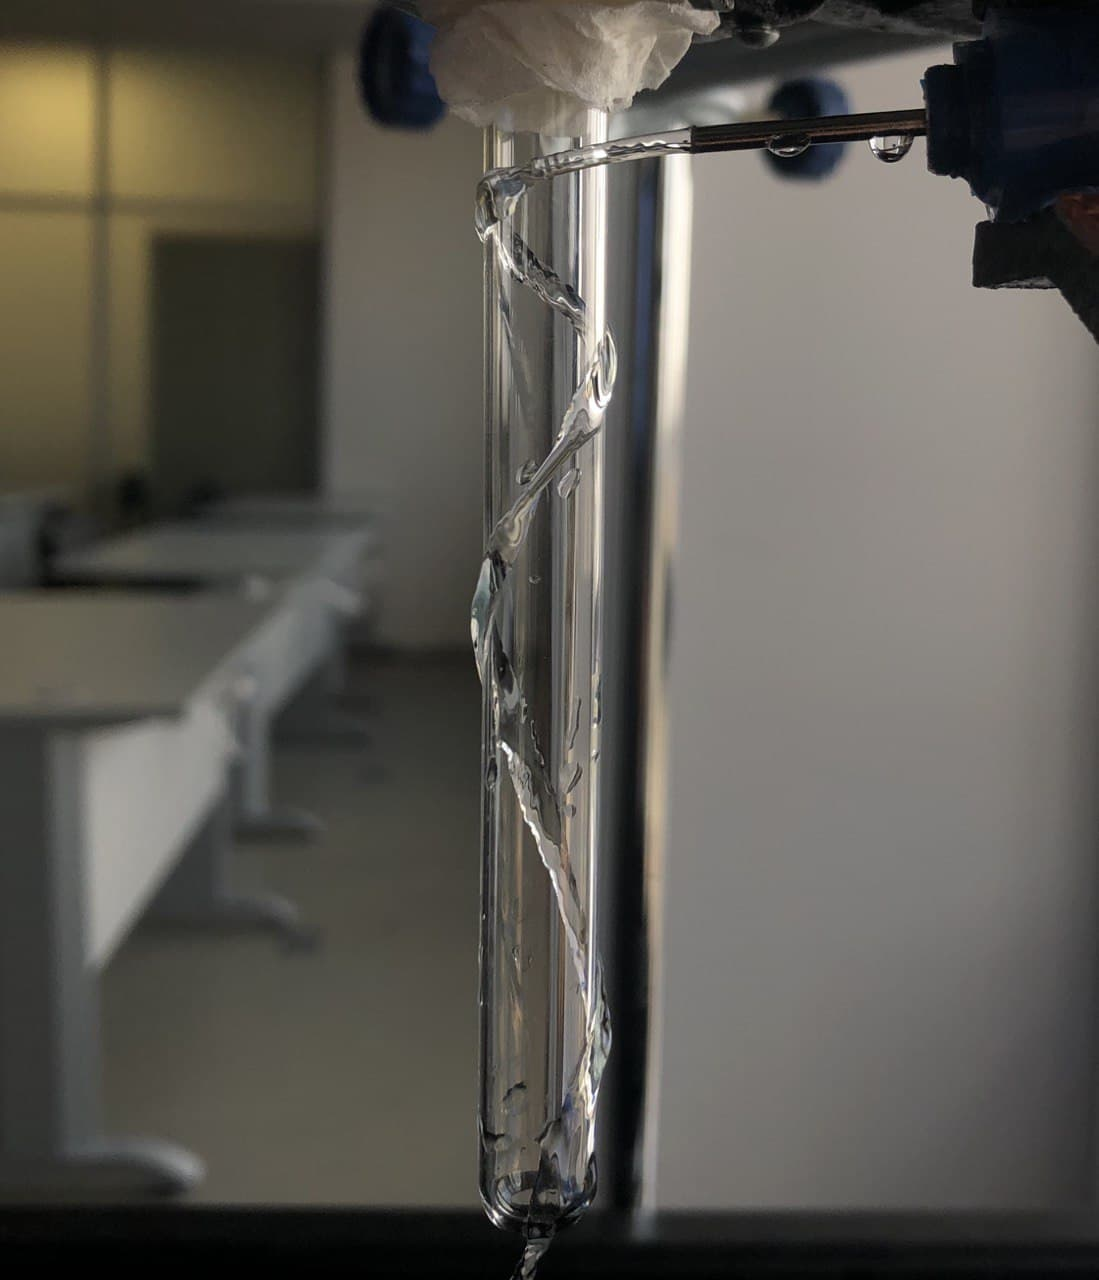
\includegraphics[width=4cm]{pic.jpg}};
    
    \begin{scope}[draw=white]
    		\dist{(0,2.57)}{(0,1.0)}{180}{left}{}
    		\path(0,{(2.57+1.0)/2}) ++ (180:.5) node [left,white] {$\lambda$};
    \end{scope}

	\end{tikzpicture}
	\end{code}
\end{minipage}
\end{figure}

	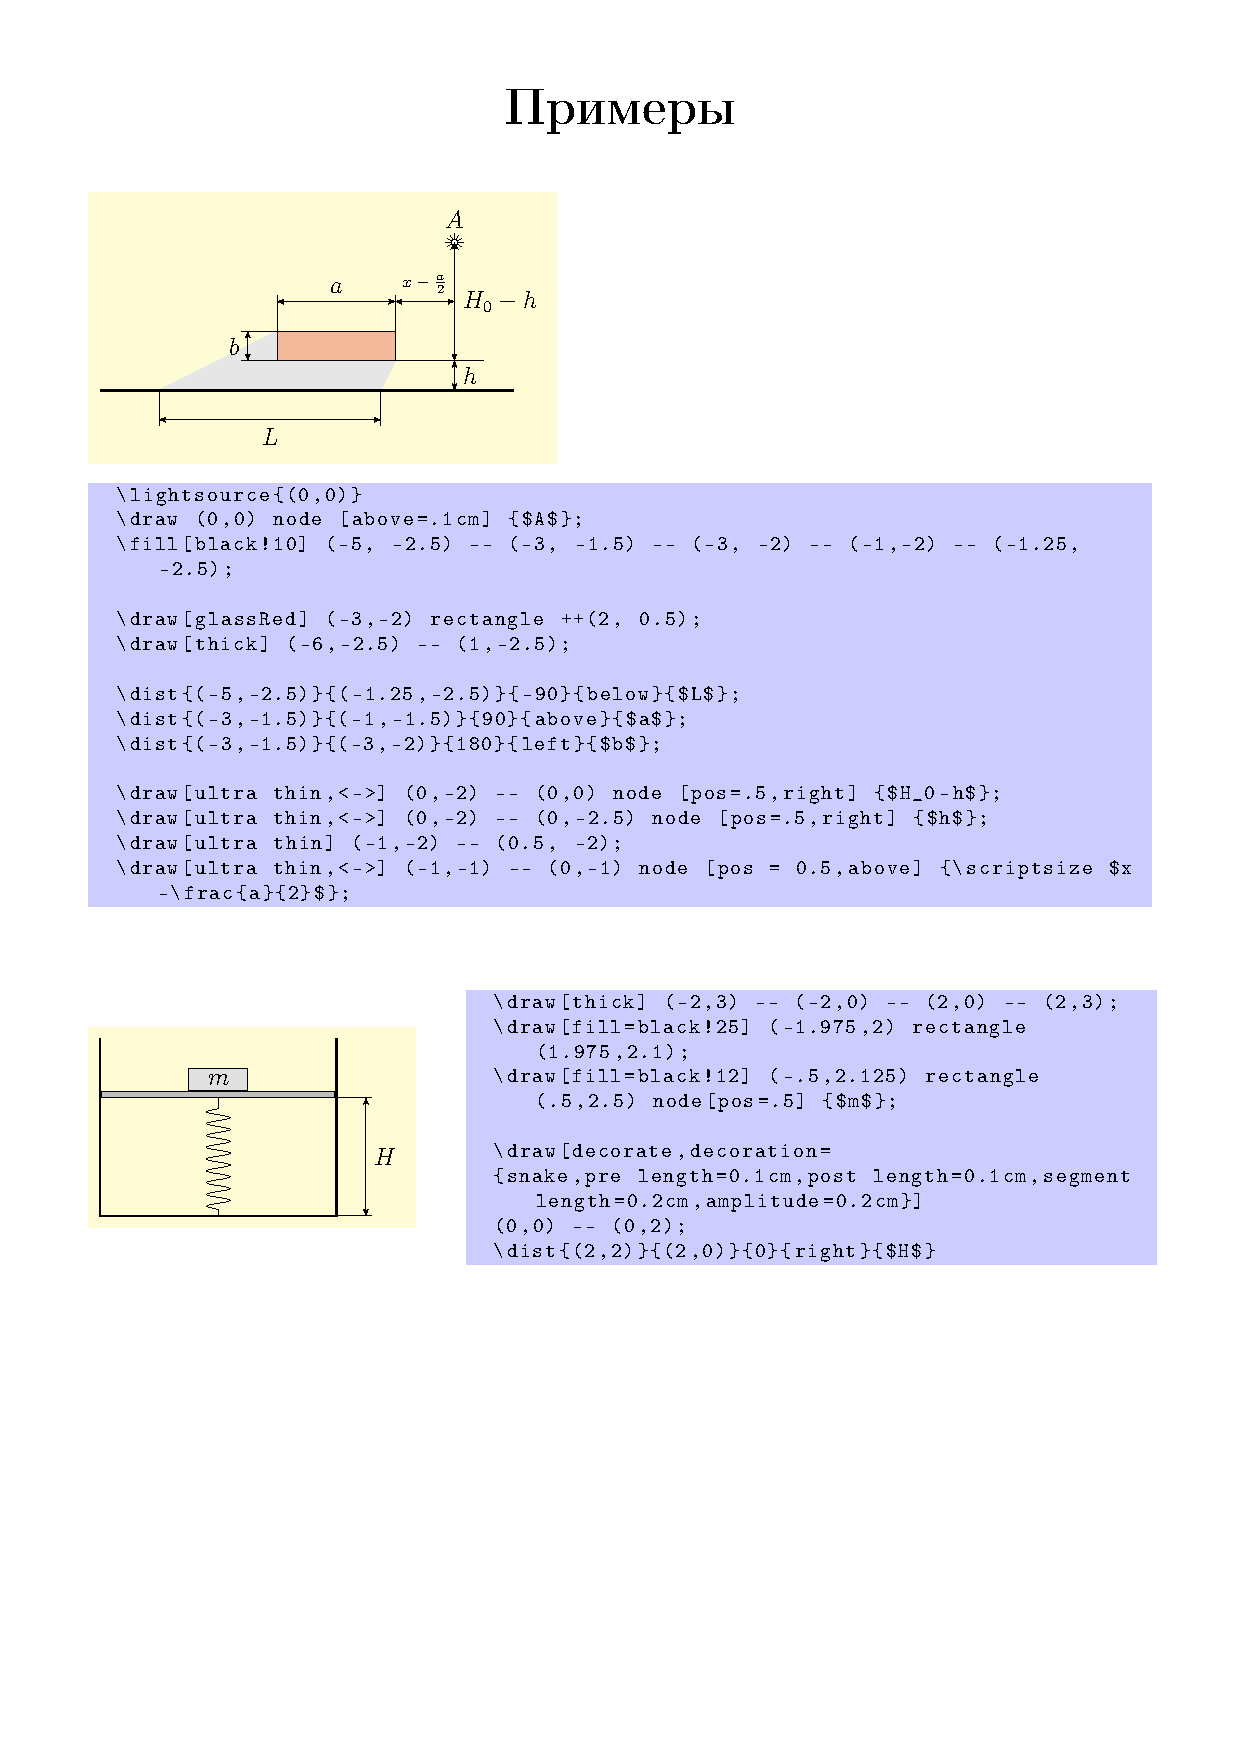
\includepdf[pages=-]{example/example.pdf}

\end{document}